

\documentclass{article}[14pt, oneside, a4paper, times]

\usepackage[utf8]{inputenc}
\usepackage[english]{babel}
\usepackage[T1]{fontenc}
\usepackage{epsfig}           % para incluir figuras
\usepackage{subfig}
\usepackage{graphicx}
\usepackage{setspace}
\usepackage{vmargin}
\usepackage{algorithm}
\usepackage{algorithmic}
\usepackage{amsfonts} 
\usepackage{amssymb}


\setpapersize [portrait]{A4}
\setmarginsrb {30mm} % margem esquerda
              {10mm} % margem topo
             {30mm} % margem direita
            {20mm} % margem pé
           {2ex}  % altura do espaco para cabeçalho
           {5ex}  % espaço entre fim do cabeçalho e início do texto
          {0pt}  % altura do espaço para rodapé
         {20mm}  % espaço entre fim do texto e fim do rodapé

\doublespacing

%=======================================================================
\pagestyle{myheadings}
\begin {document}

\title{Handwriting recognition, authenticity verification, and assurance of integrity of scanned documents 
\\ \large Review of the Literature on Month Word Recognition}
\author{Luiz S. Oliveira  
\\
\vspace {-10pt}
Federal University of Parana (UFPR)\\
\vspace {-10pt}
Department of Informatics (DInf)\\
\vspace {-10pt}
R. Rua Cel. Francisco H. dos Santos, 100, Curitiba, PR, Brazil \\
lesoliveira@inf.ufpr.br \\ 
}


\date{}
\maketitle
%\vspace{-2\baselineskip}
\thispagestyle{empty}

%\begin{abstract}

%bla bla


%\end{abstract}

%%%%%%%%%%%%%%%%%%%%%%%%%%%%%%%%%%%%%%%%%%%%%%%%%%%%%%%%%%%%%%%%%%%%%%%%%%%%%%%%%
% Introduction 
%%%%%%%%%%%%%%%%%%%%%%%%%%%%%%%%%%%%%%%%%%%%%%%%%%%%%%%%%%%%%%%%%%%%%%%%%%%%%%%%%
\section{Introduction} 

Writing, which has been the most natural mode of collecting, storing, and transmitting information through the centuries, now serves not only for communication among humans but also serves for communication of humans and machines. Machine simulation of human reading has been the subject of intensive research for the last four decades. However, the early investigations were limited by the memory and power of the computer available at that time. With the explosion of information technology, there has been a dramatic increase of research in this field since the beginning of 1980s. The interest devoted to this field is not explained only by the exciting challenges involved, but also the huge benefits that a system, designed in the context of a commercial application, could bring.

Each day, billions of business and financial documents have to be processed by computer. The great bulk of them are still processed manually by human operators, the most common and labor-consuming operation being document amount reading and typing. A common way to automate this process is to replace the human operator with an off-line recognition system that is able to do the operator's job.

With respect to document processing, many systems have been developed for information extraction, numerical string recognition, word recognition, and signature verification. Comparatively, there is very limited published work on the processing of date information even though this is a necessity in some application environments, e.g., in some countries it is illegal to process post-dated cheques.  

The main objective of this report is to present the state of the art on handwritten month recognition, which is a specific application of handwritten word recognition. Therefore, before discussing the specific application of month recognition, we present an overview of word recognition so that we can have a better understanding of the research problem. We conclude this report by outlining some of the next steps for the current project.


\section{Handwritten Word Recognition}

The majority of research in handwritten word recognition has integrated the lexicon as constraint to build lexicon-driven strategies in opposite to handwritten digit string recognition. The lexicon is a list of all valid words that are expected to be recognised by the system. There are no established definitions, however, the following terms are usually used \cite{Koerich2003}:


\begin{itemize}
\item small vocabulary - tens of words
\item medium vocabulary - hundreds of words
\item large vocabulary - thousands of words
\item very large vocabulary - tens of thousands of words
\end{itemize}


The lexicon is a key point to the success of such recognition systems, because it is a source of linguistic knowledge that helps to disambiguate single characters by looking at the entire context \cite{Kimura93}. As the number ofwords in the lexicon grows, the more difficult the recognition task becomes, because more similar words are more likely to be present in the lexicon. Koerich et al. \cite{Koerich2005} show (Figure \ref{fig:lexicon}) that, in general, the performance of the system decreases and the lexicon size gets bigger.

\begin{figure}[htbp]
   \centering
   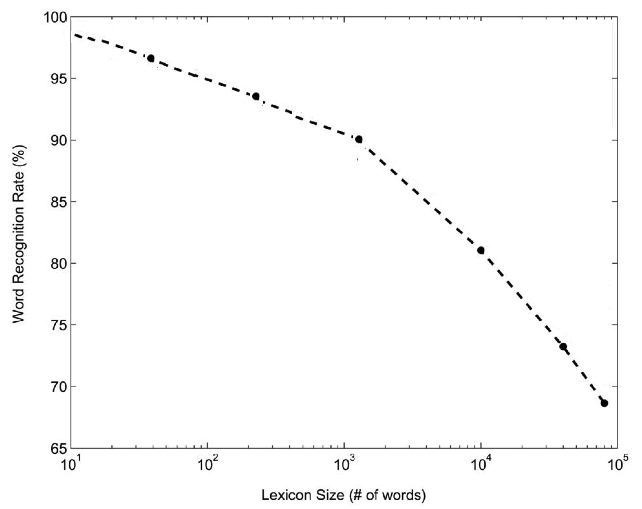
\epsfig{file=lexicon.png, width=10cm}
   \caption{Relationship between performance and the lexicon size (adapted from \cite{Koerich2005})}
   \label{fig:lexicon}
\end{figure}

Another important issue on handwritten word recognition concerns the approaches for training and recognition, which can be classified into analytic and holistic.  In an analytic approach, the segmentation of words into segments that relate to characters is required. Nevertheless, this is not a trivial task due to problems such as touching, overlapping, or broken characters. Moreover, this operation is made more difficult because of the ambiguity encountered in handwritten words. Therefore, most successful analytical methods employ segmentation-based recognition strategies where the segmentation can be explicit \cite{Arika2002, Kundu2002, ElYacoubi99, Grandidier01} or implicit \cite{Cho95, Gillies92, Mohamed96}

In an holistic approach, word recognition is performed considering the whole word. In such a case, there is no attempt to split the word image into segments. Still, it is possible that the image would be segmented in order to produce a sequence of observations \cite{Han97,Dimauro97}. 

Concerning the classification models, the literature clearly shows that the HMM (Hidden Markov Model) is the most used technique for handwritten word recognition. A HMM is a statistical Markov model in which the system being modelled is assumed to be a Markov process with unobserved (hidden) states. Even though the states are not visible in an HMM, the output that is dependent on a state is visible. Each state has a probability distribution over its possible output tokens. Therefore, the sequence of tokens generated by an HMM gives some information about the sequence of states \cite{Rabiner89,Jelinek97}.
It can be found in several different flavours combining both implicit and explicit segmentation. In Table \ref{summary-hmm:tab} we summarise some works reported in the literature that use HMM as base classifier to recognise handwritten words. 


\begin{table} [ht!]
\caption {Works using HMM to recognise handwritten words}
\begin{center}
\begin{tabular}{cccccc} \hline 
 \multicolumn{1}{c}{Ref}&
 \multicolumn{1}{c}{Lexicon}&
\multicolumn{1}{c}{Rec. Rate}&
 \multicolumn{1}{c}{Test}&
 \multicolumn{1}{c}{Database} \\
 \multicolumn{1}{c}{}&
 \multicolumn{1}{c}{Size}&
\multicolumn{1}{c}{(\%)}&
 \multicolumn{1}{c}{Set}&
 \multicolumn{1}{c}{} \\ \hline

Freitas \cite{Freitas01}  & 39    & 70 & 2380 & Legal Amount \\
Mohamed \cite{Mohamed96} &  100   & 89 & 317 & City names \\
Kundu \cite{Kundu2002} &  100   & 88 & 3,000 & City names \\
Yacoubi \cite{ElYacoubi99} &  100 & 96 & 4,313 & City names \\
Bunke \cite{Bunke95}    &  150  & 98 & 3,000 & English words \\
Arika \cite{Arika2002}  & 1,000 & 90 & 2,000 & English words \\
Gimenez \cite{Gimenez2009}& 1,117 & 70 & 14,000 & English words \\
Koerich \cite{Koerich2005}& 80.000& 68 &  4,674 & French city names \\ \hline
 
\end{tabular}
\label{summary-hmm:tab}
\end{center}
\end{table}

A direct comparison is not possible since different lexicon sizes and databases have been considered in these works. What is interesting to notice, though, is that some applications with large lexicon achieve similar of applications with small lexicon, e.g., the first and last lines in Table \ref{summary-hmm:tab}. This can be explained in parts by the similarity of the words that belong to the lexicon and also by the quality of the handwriting. 

In spite of the good performance of the HMM as word recogniser, we can find in the literature some attempts to increase the performance of HMM-based systems by implementing hybrid approaches such as HMM-SVM \cite{Ahmad2009} and HMM-Statistical Language Models \cite{Marti01}.

\section{Month Recognition}

Most of the works available in the literature on month recognition are related to Date Recognition on bank checks. Automatic reading of bank checks still is a important application since millions of bank checks issued from thousands of banks and financial institutions are daily used over the world for monetary transactions.  Thus, a machine capable of reading bank cheques will have wide applications in banks and those companies where huge quantities of cheques have to be processed since most of the cheques are still processed manually by human operators. Usually, bank cheque processing is performed in big centers or at branch agencies which are equipped with fast scanners/sorters, archiving systems, and videocoding terminals for operators who make data entry. Operators look at cheque images one by one and enter the cheque amounts.

One may find in the literature dozens of works related to the processing of courtesy and legal amounts, however, the number of works dealing with date recognition is quite limited. A recent review on automatic processing of handwritten bank cheques by Jayadevan et al \cite{Jayadevan2012} highlights this difference showing that most of the works on months recognition deal with Brazilian and Canadian bank cheques. One explanation for the lack of works on date recognition may be found in \cite{Houle1996}, where the authors state that date processing of bank cheques is considered as the most difficult target in cheque processing because of the worst segmentation and recognition performance.  

To the best of our knowledge, the first work for month recognition was proposed by Fan et al \cite{Fan96} in 1996. In this work the authors proposed a system based on HMM and neural networks to read the date field in Canadian bank cheques. They reported a very poor recognition rate at the time, around 22\% of recognition rate. One justification for such a poor performance was the huge number of ways a date can be written on a Canadian bank cheque (Figure \ref{canadiandates:fig}).  

\begin{figure}[htbp]
   \centering
   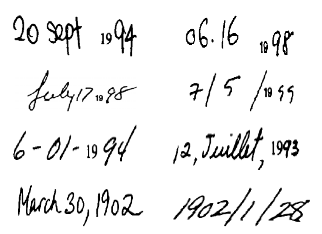
\epsfig{file=canadiandate.png, width=5cm}
   \caption{Variability of dates on Canadian bank cheques.}
   \label{canadiandates:fig}
\end{figure}

Xu et al \cite{Xu2002} pursued the work of Fan et al. and proposed a more robust month word recogniser based on HMM and two different architectures of neural networks (Multi-Layer Perceptron - MLP). They tried different combination rules including Majority Voting, Sum, and Product to fuse the outputs of the different classifies and present a recognition rate of 85.3\% on a database of 2,063 Canadian bank cheques. In \cite{Xu2003}, Xu et al. described a complete data recognition system using the month recogniser presented in \cite{Xu2002}.

Morita et al \cite{Morita2000} presented a system to recognise month words on Brazilian cheques based on a combination of holistic and analytical approaches with a single explicit segmentation technique to provide a grapheme sequence for the HMM of each recogniser. In order to perform the segmentation, first the word was divided into zones (lower, middle and upper) and then segmentation points were detected based on contour information, as depicted in Figure \ref{featureextraction:fig}. In this work they reached a recognition rate of 83.6\% on 2,000 images of Brazilian cheques.

\begin{figure}[htbp]
   \centering
   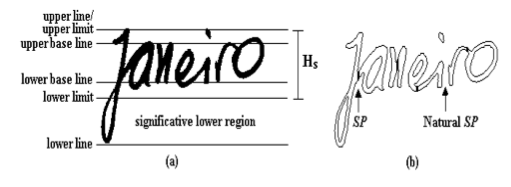
\epsfig{file=featureextraction.png, width=10cm}
   \caption{Segmentation used for feature extraction in \cite{Morita2000}.}
   \label{featureextraction:fig}
\end{figure}


Aiming at improving the results presented in \cite{Morita2000}, the authors \cite{Morita2001,Morita2004} introduce some modifications in their approach. First, in order to cope with the limited number of samples available for training, they added the legal amount database to increase the frequency of characters in training and validation sets. For this reason, in this work they have opted by the analytical approach. A feature set based on concavity analysis was used to improve the discrimination among several writing styles and then combined with global features through HMMs. In this way, a word image is represented by two feature sequences of equal length to feed the HMMs (Figure \ref{twosequences:fig}). Experiments show that this new approach reached an recognition rate of 91\% on the same 2,000 images of Brazilian bank cheques.

\begin{figure}[htbp]
   \centering
   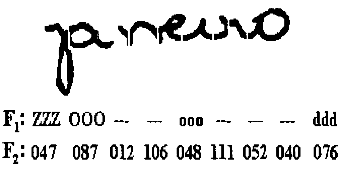
\epsfig{file=pair.png, width=7cm}
   \caption{Pair of feature sequences representing a word image \cite{Morita2001}}
   \label{twosequences:fig}
\end{figure}


Kapp et al \cite{Kapp2007} assessed two architectures of artificial neural networks for the classification of handwritten month words on Brazilian bank cheques. The performances of conventional and class-modular MLP architectures are compared. Using global features (holistic approach) like perceptual features and characteristics based on concavities/convexities, it has been found that the class-modular architecture is superior to the conventional MLP architecture. The authors reported an accuracy of 81.7\% on a database composed of 6,000 month word images.  Table \ref{summary-month:tab} summarises the aforementioned works on month recognition. 


\begin{table} [ht!]
\caption {Summary of works on month recognition}
\begin{center}
\begin{tabular}{cccccc} \hline 
 \multicolumn{1}{c}{Ref}&
 \multicolumn{1}{c}{Data set}&
\multicolumn{1}{c}{Cheque }&
 \multicolumn{1}{c}{Techniques}&
 \multicolumn{1}{c}{Recognition} \\
 \multicolumn{1}{c}{}&
 \multicolumn{1}{c}{Size}&
\multicolumn{1}{c}{Type}&
 \multicolumn{1}{c}{}&
 \multicolumn{1}{c}{Rate (\%)} \\ \hline

Fan \cite{Fan96}      & 4,565  & Canadian  & HMM,MLP & 21.8 \\
Xu \cite{Xu2002}     & 2,063  & Canadian  & HMM,MLP & 85.3 \\
Morita \cite{Morita2000} & 2,000  & Brazilian & HMM     & 83.6 \\
Morita \cite{Morita2001} & 2,000  & Brazilian & HMM     & 91.0 \\
Kapp \cite{Kapp2007}   & 6,000  & Brazilian & MLP     & 81.7 \\ \hline
 
\end{tabular}
\label{summary-month:tab}
\end{center}
\end{table}


\section{Conclusions and Further Developments}

In this report we have reviewed the literature on handwritten word recognition with focus on month word recognition. As mentioned before, most of the works on month word recognition are presented in the context of date recognition on bank cheques. The recent review presented by Jayadevan et al in \cite{Jayadevan2012} shows that the amount of works on month recognition is quite scarce when compared with the works related to other parts of the bank cheque, such as legal amount, courtesy amount, and signature verification. It  does not mean, though, that this is a less important application. On the contrary, it is very important in application environments were cheques cannot be processed prior to the dates shown. 

In spite of the limited number of works, this review give us some insights about the further developments of this project. In a first moment we intend to implement the system described in Morita et al. in \cite{Morita2001,Morita2004}, which includes the following steps:

\begin{itemize}
\item Preprocessing: Binarization, Slant Correction, Line Detection/Elimination, and Contour Smoothing. 
\item Word Segmentation into Graphemes: Segmentation step  that provides a sequence of graphemes where each one consists of a correctly segmented, an under-segmented, or a over-segmented character.
\item Feature Extraction: Two feature extractors will be implemented - Global Features and Concavity descriptors. It has been proved that both descriptors combined provide good results.  
\item Classification: The classification will be performed through HMMs. However, other classifiers will be assessed and combined with the HMMs so that we can benefit from the different classifier's architecture. 
\end{itemize}


\bibliographystyle{IEEEbib}
\bibliography{refer}



\end{document}



